\section{Results, controls, uncertainty and failure analysis}
\label{sec:results}

All numbers in this section are \textbf{[Measured]} unless marked otherwise. Every table is produced by
\texttt{python run\_all.py --stage eval report} followed by \texttt{python report/make\_tables.py}.

\subsection{Reproduction of zero-shot ESC-50 accuracy}

\begin{table}[H]
\centering\small
\caption{\textbf{[Measured]} zero-shot top-1 accuracy (\%) of the four released checkpoints with three prompts.
``Fold mean $\pm$ sd'' is over the five official folds. For comparison \textbf{[Reported]}: paper Table~4 gives 89.1 (CLAP), 88.0 (+fusion), 91.0 (+K2C);
the README gives fold-1 R@1 of 92.75 for \texttt{630k-audioset-best} and 90.50 for \texttt{630k-audioset-fusion-best} with the first prompt.}
\label{tab:repro}
\resizebox{\linewidth}{!}{\begin{tabular}{llrrrr}
\toprule
Checkpoint & Prompt & All 2000 & Fold mean $\pm$ sd & Fold-1 R@1 & Fold-1 R@5 \\
\midrule
\texttt{630k-best} & \texttt{This is a sound of \{\}.} & 90.95 & 90.95 $\pm$ 0.69 & 91.50 & 99.50 \\
\texttt{} & \texttt{This a sound of \{\}.} & 91.05 & 91.05 $\pm$ 1.27 & 92.50 & 99.75 \\
\texttt{} & \texttt{\{\}} & 84.90 & 84.90 $\pm$ 2.68 & 85.75 & 96.75 \\
\texttt{630k-audioset-best} & \texttt{This is a sound of \{\}.} & 92.30 & 92.30 $\pm$ 1.20 & 93.25 & 100.00 \\
\texttt{} & \texttt{This a sound of \{\}.} & 91.35 & 91.35 $\pm$ 1.02 & 92.25 & 100.00 \\
\texttt{} & \texttt{\{\}} & 82.05 & 82.05 $\pm$ 2.05 & 82.75 & 94.75 \\
\texttt{630k-fusion-best} & \texttt{This is a sound of \{\}.} & 91.50 & 91.50 $\pm$ 1.00 & 91.75 & 99.25 \\
\texttt{} & \texttt{This a sound of \{\}.} & 91.95 & 91.95 $\pm$ 1.58 & 91.00 & 99.50 \\
\texttt{} & \texttt{\{\}} & 83.00 & 83.00 $\pm$ 1.51 & 85.00 & 95.50 \\
\texttt{630k-audioset-fusion-best} & \texttt{This is a sound of \{\}.} & 90.80 & 90.80 $\pm$ 1.70 & 92.75 & 99.25 \\
\texttt{} & \texttt{This a sound of \{\}.} & 88.30 & 88.30 $\pm$ 1.87 & 90.25 & 99.00 \\
\texttt{} & \texttt{\{\}} & 85.20 & 85.20 $\pm$ 2.31 & 87.75 & 95.00 \\
\bottomrule
\end{tabular}}
\end{table}

\paragraph{E1 (accuracy level): confirmed.}
With the README prompt the four checkpoints reach \repbestA--\repaudiosetA\% on all 2000 clips, at or above the paper's 88.0--91.0\%.
For the pip default \texttt{630k-audioset-best}, fold-1 R@1 is \repfoldaudiosetA\% against 92.75\% in the README, a difference of one or two clips out of 400.
For the fusion default the gap is larger (\repfoldaudiosetfusionA\% vs.\ 90.50\%, 9 clips). I could not explain it: the checkpoint hash, package version and prompt are fixed,
and fusion is bypassed for 5\,s clips, so the remaining suspects are the authors' FLAC/webdataset pre-processing and the exact clip list of their ``first split''.
Since the measured number is \emph{higher}, it does not undermine the claim, but it shows that $\pm$2 points between runs of ``the same'' model can come from the pipeline alone.

\paragraph{E2 (fusion): confirmed.}
Fusion vs.\ non-fusion is $+0.55$ points for the LAION-630K pair (\repfusionA\ vs.\ \repbestA) and $-1.50$ for the AudioSet pair (\repaudiosetfusionA\ vs.\ \repaudiosetA).
Both differences are within about one fold standard deviation and have opposite signs, which matches the code reading that the fusion branch is never used for 5\,s clips.
\textbf{[Interpretation]} The paper's 89.1 vs.\ 88.0 on ESC-50 should therefore be read as a difference between two training runs, not as an effect of fusion.

\paragraph{E3 (AudioSet + K2C): not confirmed.}
Adding AudioSet with keyword-to-caption captions changes accuracy by $+1.35$ points without fusion and $-0.70$ with fusion. The paper reports $+1.9$ (89.1 to 91.0).
With released checkpoints I cannot isolate K2C, so this is weak evidence either way.

\paragraph{E4 (prompts): confirmed, and large.}
Using the bare class name instead of a sentence costs 5.6--10.3 points for every checkpoint. The paper's typo prompt is within one point of the README prompt except for the AudioSet-fusion checkpoint ($-2.5$).
Prompt choice therefore matters as much as the checkpoint choice, and cross-paper comparisons that use different prompts (Table~\ref{tab:matrix}) are not like-for-like.

\subsection{Zero-shot accuracy under background noise}

Figure~\ref{fig:snr} (blue curves) shows that zero-shot accuracy falls from \acczsKsixteenclean\% on clean audio to \acczsKsixteenwhitezerodb\% at white 0\,dB and \acczsKsixteenpinkzerodb\% at pink 0\,dB.
Brown noise has almost no effect even at 0\,dB (\acczsKsixteenbrownzerodb\%). This is a property of my corruption, not robustness of the model:
the SNR is defined over the full band, but the model only sees 50\,Hz--14\,kHz (mel filterbank of HTSAT-tiny), and only 0.3\% of brown-noise power lies in that band
(\texttt{scripts/noise\_band\_power.py}), so ``brown 0\,dB'' is about 25\,dB in-band. For white and pink noise the in-band SNR is only 2--3\,dB above nominal.
I therefore treat brown noise as a near-clean condition and base robustness conclusions on white (seen) and pink (unseen) noise.

Under strong noise the model does not fail randomly: it \emph{collapses} onto a few noise-like classes (Table~\ref{tab:collapse}).
At white 0\,dB, 25\% of all clips are labelled \emph{rain}, \emph{water drops} or \emph{vacuum cleaner}.
\textbf{[Interpretation]} The text prompts for these classes describe broadband hiss, so a hissy embedding is closest to them; this is exactly the shift a noisy cache can capture.

\begin{figure}[H]
\centering
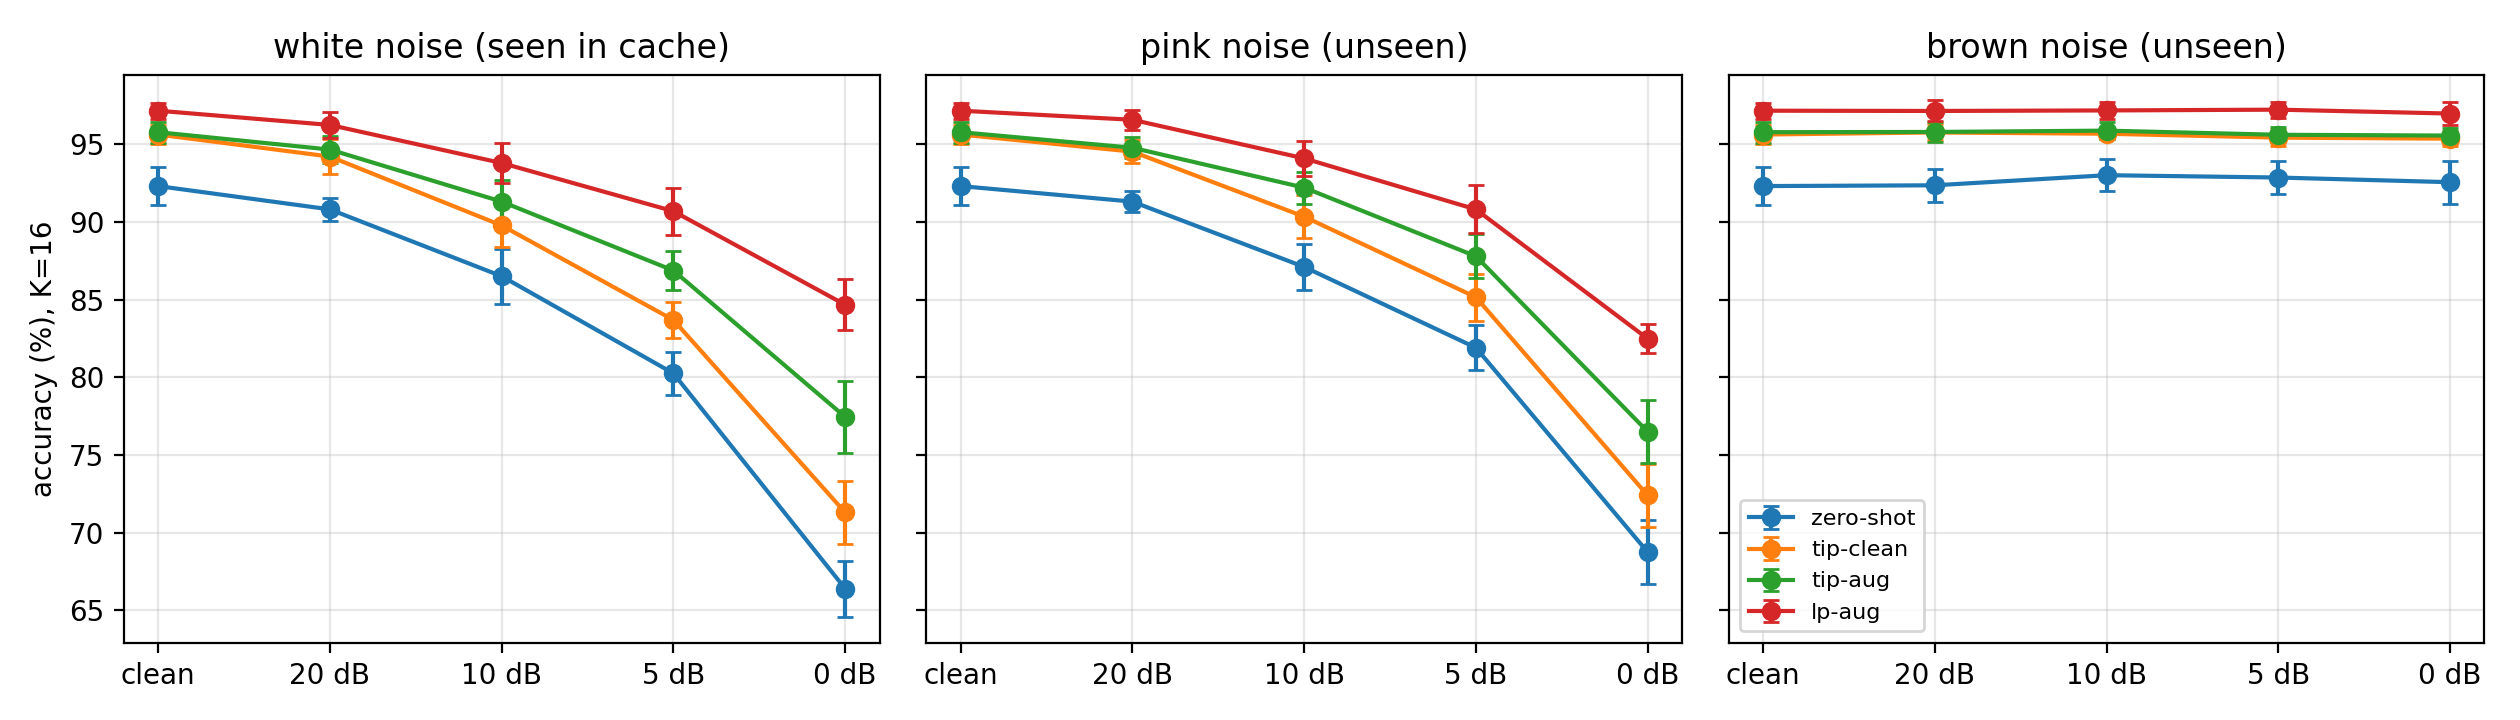
\includegraphics[width=\linewidth]{fig1_acc_vs_snr.png}
\caption{\textbf{[Measured]} accuracy vs.\ SNR with $K{=}16$ (pre-specified grid). Error bars: standard deviation over 15 runs (zero-shot: 5 folds). Only white noise was used to build the noisy cache.}
\label{fig:snr}
\end{figure}

\subsection{Noise-augmented cache vs.\ controls (pre-specified protocol)}

\begin{table}[H]
\centering\small
\caption{\textbf{[Measured]} accuracy (\%) averaged over the SNRs of each noise type, mean over 15 runs. Hyper-parameters from the pre-specified grid, selected on the clean validation fold. Bold: best per column within each $K$.}
\label{tab:main}
\begin{tabular}{lrrrrrr}
\toprule
Method & $K$ & Clean & White avg & Pink avg & Brown avg & Noisy avg \\
\midrule
Zero-shot & -- & 92.3 & 81.0 & 82.3 & 92.7 & 85.3 \\
\midrule
Tip (clean cache) & 1 & 92.8 & 81.3 & 82.5 & 93.0 & 85.6 \\
Tip (clean+noisy) \textbf{[ours]} & 1 & \textbf{93.0} & \textbf{82.0} & \textbf{83.0} & \textbf{93.2} & \textbf{86.1} \\
Tip (noisy only) & 1 & 92.8 & 81.5 & 82.7 & 93.0 & 85.7 \\
LP (clean) & 1 & 87.1 & 73.8 & 74.9 & 87.4 & 78.7 \\
LP (clean+noisy) & 1 & 87.7 & 78.9 & 79.8 & 87.6 & 82.1 \\
\midrule
Tip (clean cache) & 4 & 93.6 & 82.4 & 83.5 & 93.7 & 86.5 \\
Tip (clean+noisy) \textbf{[ours]} & 4 & 94.3 & 84.6 & 85.4 & 94.4 & 88.1 \\
Tip (noisy only) & 4 & 93.3 & 83.4 & 84.2 & 93.5 & 87.0 \\
LP (clean) & 4 & \textbf{95.7} & 83.8 & 84.5 & 95.4 & 87.9 \\
LP (clean+noisy) & 4 & 95.5 & \textbf{89.0} & \textbf{88.9} & \textbf{95.5} & \textbf{91.1} \\
\midrule
Tip (clean cache) & 16 & 95.6 & 84.7 & 85.6 & 95.5 & 88.6 \\
Tip (clean+noisy) \textbf{[ours]} & 16 & 95.8 & 87.6 & 87.8 & 95.7 & 90.4 \\
Tip (noisy only) & 16 & 95.0 & 87.5 & 87.8 & 95.0 & 90.1 \\
LP (clean) & 16 & \textbf{97.3} & 85.1 & 85.9 & 97.0 & 89.3 \\
LP (clean+noisy) & 16 & 97.2 & \textbf{91.3} & \textbf{91.0} & \textbf{97.1} & \textbf{93.1} \\
\bottomrule
\end{tabular}
\end{table}

\begin{table}[H]
\centering\small
\caption{\textbf{[Measured]} paired differences at $K{=}16$ in percentage points (same fold, seed and support set). 95\% $t$-interval over 15 runs; last column counts runs that improved / got worse.}
\label{tab:paired}
\begin{tabular}{lrlrrc}
\toprule
Comparison & $K$ & Noise & $\Delta$ (pp) & 95\% CI & better/worse runs \\
\midrule
Tip-aug - Tip-clean & 16 & brown & +0.15 & [-0.09, +0.40] & 9/6 \\
 & 16 & clean & +0.15 & [-0.10, +0.40] & 9/3 \\
 & 16 & pink & +2.21 & [+1.74, +2.68] & 15/0 \\
 & 16 & white & +2.83 & [+2.28, +3.38] & 15/0 \\
\midrule
LP-aug - LP-clean & 16 & brown & +0.15 & [-0.12, +0.41] & 8/6 \\
 & 16 & clean & -0.12 & [-0.41, +0.18] & 5/6 \\
 & 16 & pink & +5.11 & [+4.41, +5.80] & 15/0 \\
 & 16 & white & +6.21 & [+5.38, +7.03] & 15/0 \\
\midrule
Tip-clean - zero-shot & 16 & brown & +2.86 & [+2.32, +3.39] & 15/0 \\
 & 16 & clean & +3.32 & [+2.60, +4.04] & 15/0 \\
 & 16 & pink & +3.34 & [+3.02, +3.65] & 15/0 \\
 & 16 & white & +3.75 & [+3.51, +3.99] & 15/0 \\
\midrule
Tip-aug - zero-shot & 16 & brown & +3.01 & [+2.44, +3.59] & 15/0 \\
 & 16 & clean & +3.47 & [+2.68, +4.25] & 15/0 \\
 & 16 & pink & +5.55 & [+5.08, +6.02] & 15/0 \\
 & 16 & white & +6.58 & [+6.01, +7.15] & 15/0 \\
\midrule
Tip-noisy-only - Tip-clean & 16 & brown & -0.51 & [-0.67, -0.34] & 1/14 \\
 & 16 & clean & -0.57 & [-0.80, -0.33] & 1/12 \\
 & 16 & pink & +2.18 & [+1.82, +2.53] & 15/0 \\
 & 16 & white & +2.79 & [+2.30, +3.28] & 15/0 \\
\midrule
Tip-aug - LP-aug & 16 & brown & -1.42 & [-1.86, -0.98] & 0/15 \\
 & 16 & clean & -1.38 & [-1.84, -0.93] & 0/15 \\
 & 16 & pink & -3.17 & [-3.60, -2.74] & 0/15 \\
 & 16 & white & -3.77 & [-4.41, -3.14] & 0/15 \\
\bottomrule
\end{tabular}
\end{table}

\paragraph{P1 (noisy cache beats clean cache under noise): confirmed.}
At $K{=}16$ the noisy cache improves white-noise accuracy by \dtipaugvstipcleanKsixteenwhite\ points \citipaugvstipcleanKsixteenwhite\ and pink-noise accuracy by
\dtipaugvstipcleanKsixteenpink\ \citipaugvstipcleanKsixteenpink, in all 15 runs. The gain grows as SNR falls: at white 0\,dB accuracy goes from
\acctipcleanKsixteenwhitezerodb\% to \acctipaugKsixteenwhitezerodb\% (Figure~\ref{fig:snr}). At $K{=}4$ the gains are \dtipaugvstipcleanKfourwhite\ (white) and \dtipaugvstipcleanKfourpink\ (pink); at $K{=}1$ they are small (\dtipaugvstipcleanKonewhite, \dtipaugvstipcleanKonepink).

\paragraph{P2 (gain mostly for the seen noise type): partly refuted.}
The pink-noise gain is almost as large as the white-noise gain although pink noise never entered the cache, so the cache generalises across coloured noise.
Brown noise cannot answer the question because it barely corrupts the input (previous subsection).

\paragraph{P3 (no clean-accuracy cost): confirmed.}
On clean audio the difference is \dtipaugvstipcleanKsixteenclean\ points \citipaugvstipcleanKsixteenclean\ at $K{=}16$. The \emph{noisy-only} ablation shows why the clean keys matter:
without them noisy accuracy is about the same but clean accuracy drops (\dtipnoisyonlyvstipcleanKsixteenclean\ points, \citipnoisyonlyvstipcleanKsixteenclean).

\paragraph{P4 (does the gain come from the data or from the cache?): the data, and the cache is not the best user of it.}
The linear probe gains even more from the same augmented support set (\dlpaugvslpcleanKsixteenwhite\ white, \dlpaugvslpcleanKsixteenpink\ pink at $K{=}16$),
and for $K\ge4$ the probe on clean+noisy data is the best method overall: \mainlpaugKsixteennoisy\% average noisy accuracy vs.\ \maintipaugKsixteennoisy\% for the noisy cache, and
\mainlpaugKsixteenclean\% vs.\ \maintipaugKsixteenclean\% on clean audio. Only at $K{=}1$ is the cache clearly better than the probe
(\maintipaugKoneclean\% vs.\ \mainlpaugKoneclean\% clean), because a 50-sample logistic regression has no text prior to fall back on (Figure~\ref{fig:shots}).
\textbf{This is a negative result for the cache mechanism:} noise augmentation of the support set is what helps, and with four or more clips per class a trained probe exploits it better than a training-free cache.

\begin{figure}[H]
\centering
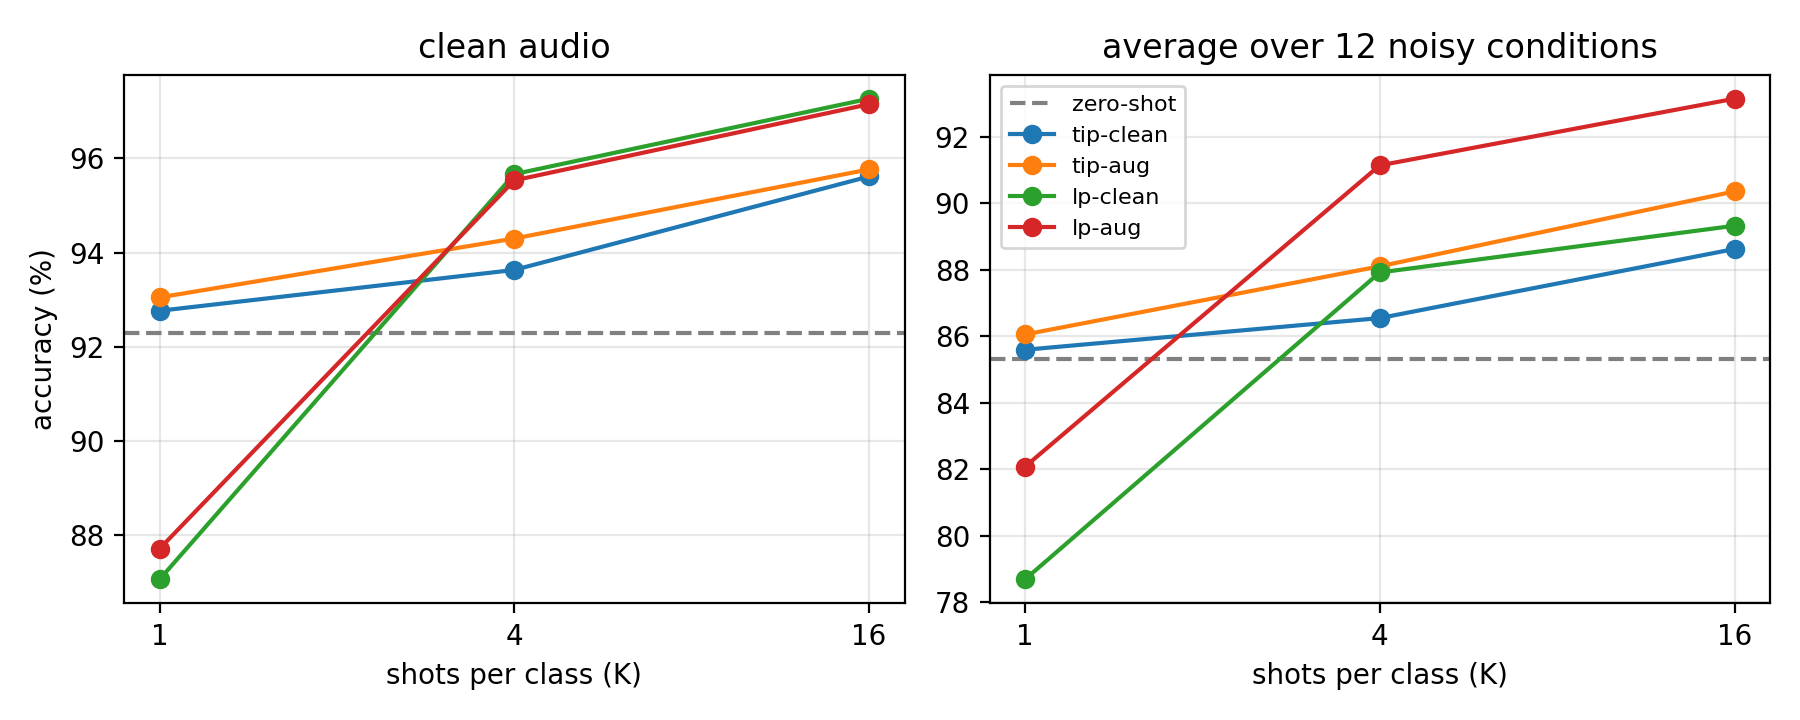
\includegraphics[width=0.9\linewidth]{fig2_acc_vs_shots.png}
\caption{\textbf{[Measured]} accuracy vs.\ shots per class, clean audio (left) and average over the 12 noisy conditions (right). Dashed line: zero-shot.}
\label{fig:shots}
\end{figure}

\subsection{Investigating the gap to the probe: the cache-weight grid was too narrow}
\label{sec:ext}
Before attributing P4 to the method I checked the selected hyper-parameters. In \mainalphaedge\ of \mainalphaN\ cache runs the validation fold selected
$\alpha=4$, the largest value in the pre-specified grid, so the cache weight was probably capped. I re-ran only the CPU stages on the saved embeddings with
$\alpha$ up to 128 and $\beta$ down to 0.25 (\texttt{configs/extended\_grid.yaml}); selection is still on the clean validation fold, and nothing else changes.
This is a follow-up decided after seeing the boundary, so I report it next to, not instead of, the pre-specified result.

\begin{table}[H]
\centering\small
\caption{\textbf{[Measured]} same as Table~\ref{tab:main} with the extended grid ($\alpha\le128$, $\beta\ge0.25$). Zero-shot and probe rows are unchanged by construction.}
\label{tab:ext}
\begin{tabular}{lrrrrrr}
\toprule
Method & $K$ & Clean & White avg & Pink avg & Brown avg & Noisy avg \\
\midrule
Zero-shot & -- & 92.3 & 81.0 & 82.3 & 92.7 & 85.3 \\
\midrule
Tip (clean cache) & 1 & 94.2 & 83.1 & 83.9 & 94.1 & 87.1 \\
Tip (clean+noisy) \textbf{[ours]} & 1 & \textbf{94.3} & \textbf{84.9} & \textbf{85.4} & \textbf{94.3} & \textbf{88.2} \\
Tip (noisy only) & 1 & 93.7 & 84.8 & 85.3 & 93.6 & 87.9 \\
LP (clean) & 1 & 87.1 & 73.8 & 74.9 & 87.4 & 78.7 \\
LP (clean+noisy) & 1 & 87.7 & 78.9 & 79.8 & 87.6 & 82.1 \\
\midrule
Tip (clean cache) & 4 & 95.3 & 85.1 & 85.4 & 95.3 & 88.6 \\
Tip (clean+noisy) \textbf{[ours]} & 4 & 95.4 & 87.9 & 87.9 & 95.4 & 90.4 \\
Tip (noisy only) & 4 & 95.2 & 88.2 & 88.2 & 95.2 & 90.5 \\
LP (clean) & 4 & \textbf{95.7} & 83.8 & 84.5 & 95.4 & 87.9 \\
LP (clean+noisy) & 4 & 95.5 & \textbf{89.0} & \textbf{88.9} & \textbf{95.5} & \textbf{91.1} \\
\midrule
Tip (clean cache) & 16 & 96.1 & 85.8 & 86.1 & 96.2 & 89.4 \\
Tip (clean+noisy) \textbf{[ours]} & 16 & 96.1 & 89.3 & 89.3 & 96.3 & 91.6 \\
Tip (noisy only) & 16 & 95.2 & 89.1 & 89.6 & 95.3 & 91.3 \\
LP (clean) & 16 & \textbf{97.3} & 85.1 & 85.9 & 97.0 & 89.3 \\
LP (clean+noisy) & 16 & 97.2 & \textbf{91.3} & \textbf{91.0} & \textbf{97.1} & \textbf{93.1} \\
\bottomrule
\end{tabular}
\end{table}

With the wider grid both caches improve (e.g.\ $K{=}16$ clean: \exttipcleanKsixteenclean\% and \exttipaugKsixteenclean\%), and the noisy-cache gain over the clean cache becomes larger:
\extdtipaugvstipcleanKsixteenwhite\ \extcitipaugvstipcleanKsixteenwhite\ points for white and \extdtipaugvstipcleanKsixteenpink\ \extcitipaugvstipcleanKsixteenpink\ for pink noise, still with no clean cost (\extdtipaugvstipcleanKsixteenclean).
The gap to the augmented probe shrinks but does not close: at $K{=}16$ the cache is still \extdtipaugvslpaugKsixteenwhite\ \extcitipaugvslpaugKsixteenwhite\ points behind on white noise and \extdtipaugvslpaugKsixteenclean\ on clean audio;
at $K{=}4$ they are tied on clean audio (\extdtipaugvslpaugKfourclean\ \extcitipaugvslpaugKfourclean). Even in this grid \extalphaedge\ of \extalphaN\ runs chose the largest $\alpha$.
\textbf{[Interpretation]} Validation keeps asking for a cache that dominates the text prior, i.e.\ once a few labelled clips exist the zero-shot term contributes little on ESC-50. So the conclusions of the previous subsection hold with either grid: the noisy cache reliably beats the clean cache, and the probe remains the stronger adapter for $K\ge4$.

\subsection{Resource cost}

The audio encoder dominates the cost: on the RTX 3080 it needs \enclatencybsonemsmedian\,ms per clip at batch size 1 (peak memory \encpeakmembsoneMB\,MB)
and \encperclipmsbatched\,ms per clip at batch size 32 (\encthroughputclipspers\ clips/s, peak \encpeakmembsthreetwoMB\,MB).
The intervention adds one encoder pass per support clip at set-up, e.g.\ 800 extra clips $\approx$ 5\,s at $K{=}16$, and doubles the cache (Table~\ref{tab:res}).
At test time the noisy cache adds about 0.006\,ms per clip on the CPU, more than 1000 times less than the encoder, so robustness comes at no meaningful run-time cost.
Probes need a few hundred milliseconds of training (with $C$ selection); caches need none.

\begin{table}[H]
\centering\small
\caption{\textbf{[Measured]} adapter cost on top of frozen embeddings (CPU, NumPy/scikit-learn, mean over runs). Tuning includes the full hyper-parameter search on the validation fold.}
\label{tab:res}
\resizebox{0.85\linewidth}{!}{\begin{tabular}{lrrrrr}
\toprule
Method & $K$ & Entries & Size (MB) & Tuning (s) & Inference (ms/clip) \\
\midrule
Zero-shot & 0 & 0 & 0.000 & 0.000 & 0.0013 \\
LP (clean+noisy) & 1 & 100 & 0.195 & 0.143 & 0.0025 \\
LP (clean) & 1 & 50 & 0.098 & 0.139 & 0.0021 \\
Tip (clean+noisy) & 1 & 100 & 0.195 & 0.002 & 0.0019 \\
Tip (clean cache) & 1 & 50 & 0.098 & 0.003 & 0.0015 \\
Tip (noisy only) & 1 & 50 & 0.098 & 0.002 & 0.0016 \\
LP (clean+noisy) & 4 & 400 & 0.781 & 0.254 & 0.0025 \\
LP (clean) & 4 & 200 & 0.391 & 0.171 & 0.0022 \\
Tip (clean+noisy) & 4 & 400 & 0.781 & 0.004 & 0.0033 \\
Tip (clean cache) & 4 & 200 & 0.391 & 0.003 & 0.0021 \\
Tip (noisy only) & 4 & 200 & 0.391 & 0.003 & 0.0023 \\
LP (clean+noisy) & 16 & 1600 & 3.125 & 0.641 & 0.0022 \\
LP (clean) & 16 & 800 & 1.562 & 0.288 & 0.0022 \\
Tip (clean+noisy) & 16 & 1600 & 3.125 & 0.017 & 0.0143 \\
Tip (clean cache) & 16 & 800 & 1.562 & 0.010 & 0.0083 \\
Tip (noisy only) & 16 & 800 & 1.562 & 0.010 & 0.0083 \\
\bottomrule
\end{tabular}}
\end{table}

\subsection{Failure analysis}

\begin{table}[H]
\centering\small
\begin{minipage}{0.44\linewidth}\centering
\caption{\textbf{[Measured]} classes with the largest zero-shot drop (clean vs.\ average of 12 noisy conditions).}
\label{tab:drop}
\begin{tabular}{lrrr}
\toprule
Class & Clean & Noisy avg & Drop (pp) \\
\midrule
laughing & 100.0 & 70.0 & 30.0 \\
airplane & 95.0 & 67.5 & 27.5 \\
train & 100.0 & 75.6 & 24.4 \\
engine & 90.0 & 67.9 & 22.1 \\
clock alarm & 100.0 & 79.0 & 21.0 \\
drinking sipping & 85.0 & 67.9 & 17.1 \\
can opening & 95.0 & 78.5 & 16.5 \\
car horn & 97.5 & 81.9 & 15.6 \\
\bottomrule
\end{tabular}
\end{minipage}\hfill
\begin{minipage}{0.52\linewidth}\centering
\caption{\textbf{[Measured]} per-class effect of the noisy cache (noisy average, $K{=}16$, seed 0): five largest gains and five largest losses.}
\label{tab:classgain}
\begin{tabular}{lrrr}
\toprule
Class & Tip clean & Tip clean+noisy & $\Delta$ \\
\midrule
wind & 43.1 & 50.2 & +7.1 \\
laughing & 71.5 & 77.7 & +6.2 \\
airplane & 65.2 & 71.5 & +6.2 \\
train & 76.5 & 81.9 & +5.4 \\
can opening & 80.4 & 84.8 & +4.4 \\
\midrule
insects & 90.6 & 90.2 & -0.4 \\
chainsaw & 92.9 & 92.5 & -0.4 \\
clock tick & 99.0 & 98.5 & -0.4 \\
vacuum cleaner & 98.1 & 97.5 & -0.6 \\
rain & 98.5 & 97.3 & -1.2 \\
\bottomrule
\end{tabular}
\end{minipage}
\end{table}

\begin{table}[H]
\centering\small
\caption{\textbf{[Measured]} prediction collapse at 0\,dB: the three most predicted classes over all 2000 clips (pre-specified grid, $K{=}16$, seed 0).}
\label{tab:collapse}
\resizebox{\linewidth}{!}{\begin{tabular}{llp{7.2cm}r}
\toprule
Method & Condition & Top-3 predicted classes (count) & Top-3 share (\%) \\
\midrule
Zero-shot & white 0dB & rain (236), water drops (156), vacuum cleaner (117) & 25.4 \\
Tip (clean+noisy) & white 0dB & rain (149), water drops (93), vacuum cleaner (90) & 16.6 \\
Zero-shot & pink 0dB & rain (231), water drops (82), vacuum cleaner (79) & 19.6 \\
Tip (clean+noisy) & pink 0dB & rain (166), wind (65), cat (65) & 14.8 \\
Zero-shot & brown 0dB & insects (55), train (53), sea waves (52) & 8.0 \\
Tip (clean+noisy) & brown 0dB & sea waves (53), train (52), airplane (46) & 7.5 \\
\bottomrule
\end{tabular}}
\end{table}

The classes hurt most by noise are sounds with tonal or narrow-band structure that broadband noise masks (\emph{laughing}, \emph{airplane}, \emph{train}, \emph{engine}, \emph{clock alarm}; Table~\ref{tab:drop}).
The noisy cache helps most on the same kind of classes and on \emph{wind}, which is itself noise-like.
Unfavourable cases exist: the classes that act as ``sinks'' under noise (\emph{rain}, \emph{vacuum cleaner}) and a few others lose about 0.4--1.2 points; \textbf{[Interpretation]} the noisy keys of other classes now compete with them in the region where they used to win by default.
Across 50 classes the noisy cache helps \nClassGain\ and hurts \nClassLoss\ (seed 0, $K{=}16$, noisy average). It also reduces the collapse: at white 0\,dB the share of the three most-predicted classes falls from 25.4\% to 16.6\% (Table~\ref{tab:collapse}).
The remaining hard case is \emph{wind}: it is weak even on clean audio (42.5\% zero-shot) and stays between 34 and 50\% under noise for every method.
